\chapter{پیاده‌سازی و توسعه مدل یادگیری ماشین}

در این فصل روش پیاده‌سازی مدل هوش مصنوعی را به تفصیل شرح خواهیم داد. ابتدا فرضیات و داده‌های ورودی و آماده‌ی تحلیل را مشخص کرده و نماد هر کدام را که تا انتهای این نوشته از آنها استفاده خواهیم کرد، مشخص می‌کنیم. در قسمت بعد مراحل پیش‌پردازش\LTRfootnote{Preprocess} را که روی این داده‌ها انجام می‌شود به ترتیب توضیح می‌دهیم و سپس ویژگی‌هایی که نیاز داریم از این داده‌های خام دربیاوریم را توضیح می‌دهیم و نحوه‌ی استخراج این ویژگی‌ها را نمایان می‌کنیم. در مرحله‌ی نهایی نحوه‌ی یادگیری مدل هوش مصنوعی و پیش‌بینی عمر باقی‌مانده‌ی دستگاه‌ها را بر اساس این ویژگی‌ها شرح می‌دهیم. در \cref{fig:analytics_structure}، قالب بسته‌ی هوش مصنوعی توسعه داده‌شده برای کارگزار اصلی را مشاهده می‌کنید که در این فصل به توضیح بخش‌های مختلف آن می‌پردازیم.

\begin{figure}[!h]
\centerline{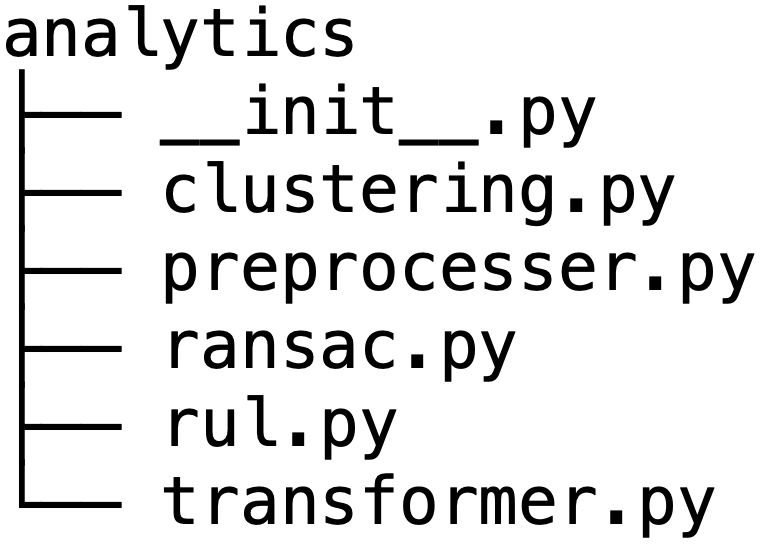
\includegraphics[width=0.4\textwidth]{analytics_structure.png}}
\caption{ساختار کلی بسته‌ی هوش مصنوعی}
\label{fig:analytics_structure}
\end{figure}


\section{توضیح مسئله}
با توجه به اینکه سیستم یادگیری ماشین بر اساس اطلاعات حسگرهای لرزش عمل می‌کند، برای داشتن کمترین خطا در عملیات پیش‌بینی باید فرضیاتی را پیش از طراحی و پیاده‌سازی سیستم در نظر داشته باشیم. اولاً نمونه‌های بدست‌آمده برای حسگرهای متفاوت بازه‌های زمانی مختلف را در بر می‌گیرند و همگن نیستند. ثانیاً این داده‌های دارای انحرافاتی در اندازه‌گیری بدلیل وجود گرانش یا خرابی حسگر هستند. ثالثاً وضعیت ابتدایی هر یک از گره‌هایی که می‌خواهیم اطلاعات لرزش آنها را جمع‌آوری و تحلیل کنیم یکی نیستند\cite{jung2017vibration}. با توجه به نکاتی که مطرح کردیم، پیاده‌کردن یک سیستم پیش‌پردازش و استخراج‌کننده‌ی ویژگی‌های مناسب، الزامی است. 

\begin{table}[h!]
  \begin{center}
    \caption{توضیحات نشانه‌گذاری داده‌ها}
    \label{table:notation_description}
    \begin{tabular}{|c|c|} % <-- Alignments: 1st column left and 2nd right with vertical lines in between
    	\hline
توضیحات & نشانه\\
    	\hline \hline
تعداد کل گره‌ها & $N$\\
    	\hline
 تعداد کل اندازه‌گیری‌ها & $M$\\
    	\hline
   تعداد کل نمونه‌های یک اندازه‌گیری & $K$\\
    	\hline
گره $n$ ام & $n$\\
 	\hline
اندازه‌گیری $m$ ام & $m$\\
 	\hline
نمونه‌ی $k$ ام یک اندازه‌گیری & $k$\\
 	\hline
بردار سه‌بعدی مربوط به اندازه‌گیری لرزش & $a_{nmk}$\\
 	\hline
بردار $k$بعدی مربوط به لرزش در محور $l \in \{x, y, z\}$  & $a^l_{nm}$\\
 	\hline
    \end{tabular}
  \end{center}
\end{table} 

\begin{table}[h!]
  \begin{center}
    \caption{برچسب‌های استفاده‌شده برای تعیین وضعیت دستگاه‌ها}
    \label{table:node_state_labels}
    \begin{tabular}{|c|c|} % <-- Alignments: 1st column left and 2nd right with vertical lines in between
    	\hline
توضیحات & برچسب\\
    	\hline \hline
دستگاه‌های نو که تازه تولید شده‌اند و آماده استفاده‌اند & $A$\\
    	\hline
دستگاه‌هایی که نو نیستند ولی هنوز مشغول کارکردن هستند & $B, C$\\
    	\hline
  دستگاه‌هایی خراب‌ شده‌اند یا در حال خرابی‌اند & $D$\\
    	\hline
    \end{tabular}
  \end{center}
\end{table}

در \cref{table:notation_description} توضیحات نشانه‌گذاری داده‌ی مربوط به این مسئله را می‌بینیم. همچنین در جهت مشخص کردن محدوده‌ی کاری این مسئله، از سه برچسب که در \cref{table:node_state_labels} مشخص شده‌اند، برای تعیین کردن وضعیت گره‌های موجود استفاده می‌کنیم.

\section{پیش‌پردازش}
این بخش وظیفه دارد قبل از انجام تحلیل داده، در ابتدا انحرافات و داده‌های پرت\LTRfootnote{Outlier Data} را از داده‌ی خام جدا کرده و داده‌ی قابل پردازش را به لایه‌ی بعد که لایه‌ی استخراج ویژگی‌ است تحویل دهد. در نهایت خروجی بخش پیش‌پردازنده، ویژگی‌هایی هستند که دستگاه یادگیری ماشین با تحلیل و بررسی آنها عملیات یادگیری و پیش‌بینی را انجام خواهد داد.

\subsection{از بین بردن انحرافات}
 حسگرهای کم‌هزینه \lr{MEMS} ،که داده‌های جمع‌آوری‌شده برای این پروژه توسط این نوع از حسگرها تأمین شده است، غالباً با گذشت زمان دچار انحرافاتی در اندازه‌گیری خواهند شد که منجر به اضافه یا کم شدن یک مقدار شتاب غیر صفر در اندازه‌گیری‌هایشان خواهد شد. از طرفی وجود گرانش، تاثیراتی روی اندازه‌گیری‌ها خواهد داشت و موجب ایجاد انحرافاتی رو به بالا یا پایین در این مقادیر خواهد شد\cite{jung2017vibration}. برای از بین بردن این مشکل همانطور که در \cref{eq:normalize} آورده شده است\cite{garcia2015data}، از هنجار‌کردن\LTRfootnote{Normalizing} داده با کم‌کردن میانگین مقادیر شتاب اندازه‌گیری شده در هر کدام از سه محور از مقادیر اندازه‌گیری‌شده استفاده کرده‌ایم. لازم به ذکر است همانطور که مشخص است، $\hat{a}^l_{nm}$ نماد ماتریس هنجار‌شده است.
\begin{equation}
\label{eq:normalize}
	\hat{a}^l_{nm}=a^l_{nm}-\sum_{k=1}^K \dfrac{a^l_{nmk}}{K}
\end{equation}


\subsection{از بین بردن داده‌های پرت}
در سیستم طراحی‌شده برای جمع‌آوری اطلاعات، ممکن است که تعدادی از حسگرها دچار مشکل شده باشند و داده‌ای که تحویل دروازه می‌دهند دقیق و در راستای داده‌های از قبل جمع‌آوری شده نباشد. به طور کلی، پایدار بودن میانگین شتاب دریافت‌شده از هر اندازه‌گیری، معیار خوبی برای تشخیص صحت و درستی اطلاعات جمع‌‌آوری شده است\cite{jung2017vibration}. به عبارتی دیگر، میانگین لرزش‌های اندازه گرفته‌شده نباید به طور ناگهانی بالا یا پایین روند و باید در همان حدود اندازه‌گیری‌های قبل باشند. برای جدا کردن این داده‌ها که اصطلاحا به آنها داده‌های پرت می‌گوییم، پیش از شروع یادگیری مدل، ابتدا میانگین شتاب جمع‌‌آوری ‌شده برای هر اندازه‌گیری موجود را در هر سه بعد حساب کرده و سپس با کمک یک الگوریتم خوشه‌بندی\LTRfootnote{Clustering}، این داده‌ها را جدا می‌کنیم.

برای انجام عملیات تشخیص داده‌های پرت، از الگوریتم خوشه‌بندی میانگین تغییر\LTRfootnote{Mean Shift} استفاده کرده‌ایم که الگوریتمی بر اساس تخمین تراکم هسته\LTRfootnote{Kernel Density Estimate} می‌باشد. در \cref{fig:density_based_clustering}\cite{carreira2015review} نمونه‌ای از یک الگوریتم خوشه‌بندی تراکم‌محور آورده شده است. روند کار این الگوریتم بدین صورت است که به ازای ورودی به صورت نقاط و پارامتر ورودی پهنای باند\LTRfootnote{Bandwidth}، الگوریتم به طور مکرر هر نقطه داده را به نزدیکترین مرکز خوشه اختصاص می‌دهد و جهت نزدیکترین مرکز خوشه بر اساس جایی که اکثر نقاط نزدیک در آن قرار دارند تعیین می‌شود. در هر بار تکرار، هر نقطه داده به جایی که بیشترین نقاط در آن قرار دارد، نزدیکتر می‌شود، که در نهایت به مرکز خوشه منجر خواهد شد. هنگامی که الگوریتم متوقف می‌شود، هر نقطه به یک خوشه اختصاص داده می‌شود. همانطور که گفته‌شد، این الگوریتم بغیر از پهنای باند به پارامتر دیگری نیاز ندارد. این امر سبب می‌شود که مواردی همانند تعداد و مراکز هر خوشه، توسط خود الگوریتم مشخص شوند\cite{carreira2015review}.

\begin{figure}[!h]
\centerline{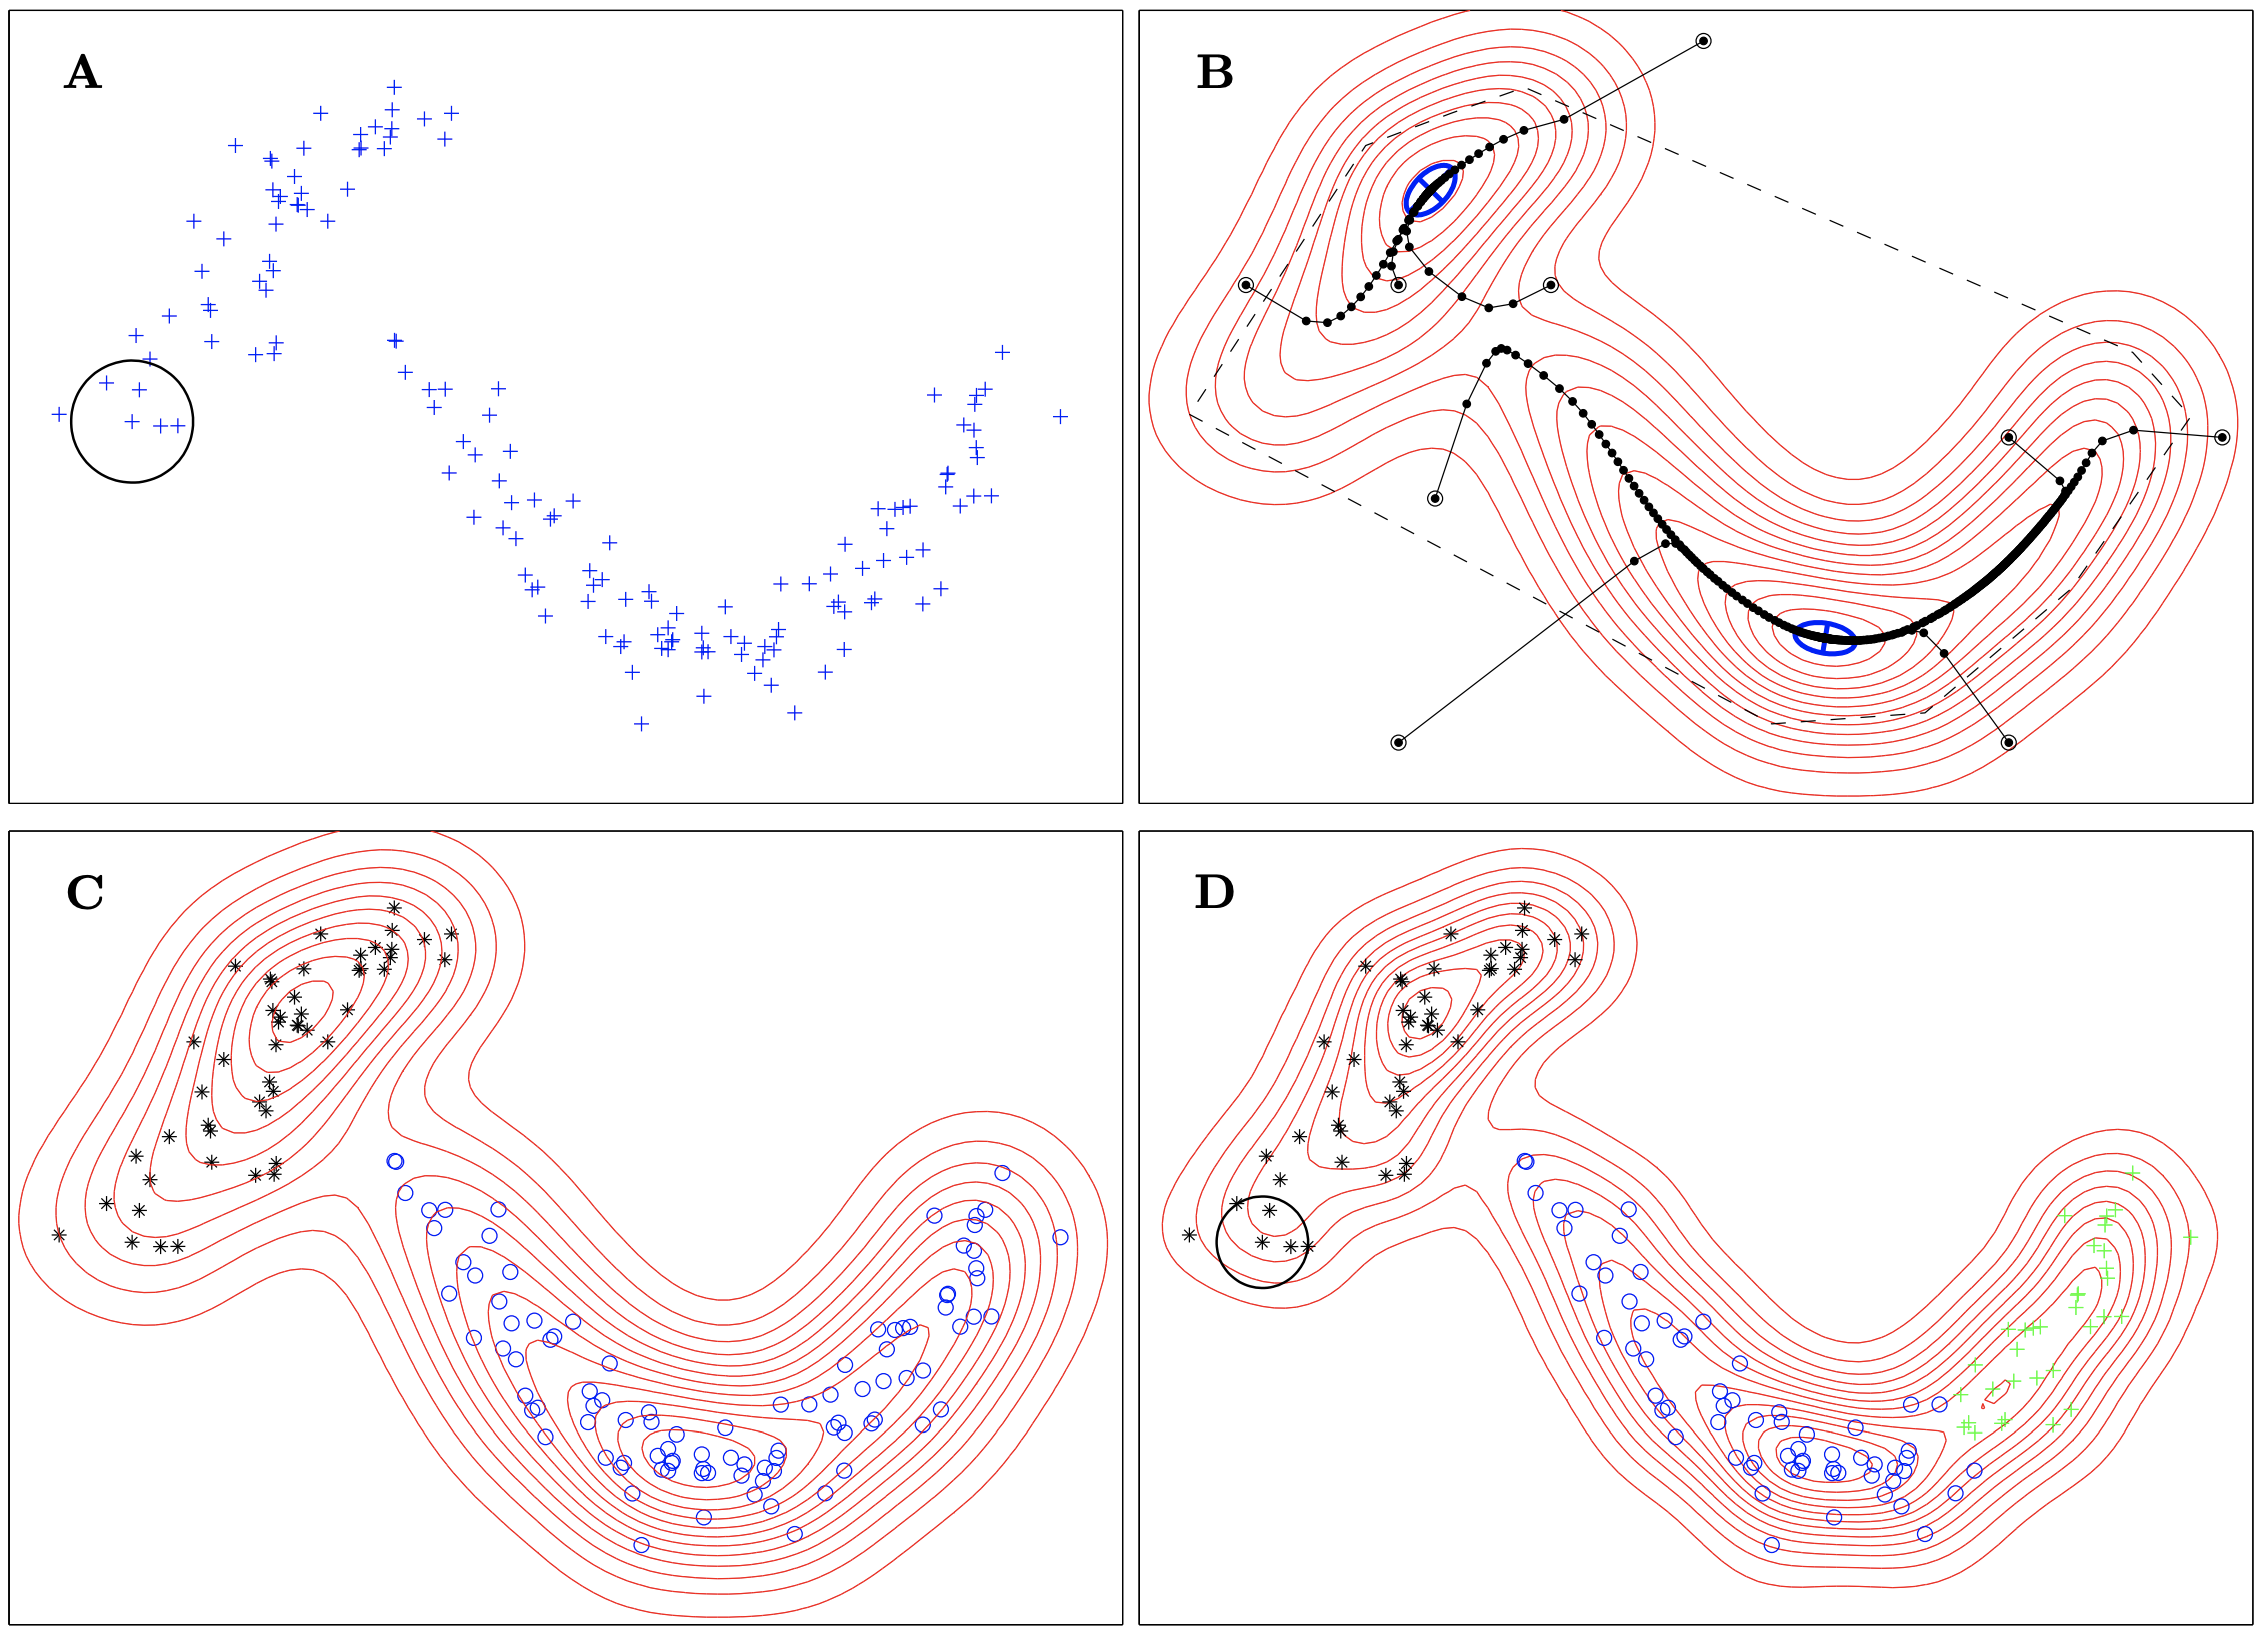
\includegraphics[width=\textwidth]{density_based_clustering.png}}
\caption{روند خوشه‌بندی یک الگوریتم تراکم‌محور\cite{carreira2015review}}
\label{fig:density_based_clustering}
\end{figure}

نحوه‌ی استفاده از این الگوریتم در این مسئله بدین گونه است که پیش از عملیات استخراج ویژگی‌ها و یادگیری ماشین، میانگین مقادیر لرزش در هر سه بعد برای هر اندازه‌گیری محاسبه می‌شود. این مقادیر نباید خیلی با هم اختلاف داشته باشند. برای تشخیص داده‌های پرت، خوشه‌بندی میانگین تغییر سه‌بعدی استفاده می‌کنیم و در نهایت داده‌هایی که در خوشه‌ی اقلیت قرار دارند را برای محاسبات و یادگیری ماشین در نظر نمی‌گیریم\cite{jung2017vibration}. برای پیاده‌سازی این الگوریتم کلاس \lr{MeanShiftClustering} در فایل \lr{clustering.py} پیاده‌شده است. این کلاس از کلاس \lr{MeanShift} از کتابخانه‌ی \lr{Scikit-Learn} ارث‌بری می‌کند.


\subsection{استخراج ویژگی‌ها}
تا اینجای کار، اثرهای انحرافات ممکن را از بین بردیم و داده‌های پرت را از میان کل داده‌ها جدا کردیم. از آنجا که داده‌ی خام لرزش گره‌های موجود در شبکه‌ی اشیاء، در دامنه‌ی زمانی\LTRfootnote{Time Domain} بوده و حالت شروع به کار و وضعیت فعلی هر کدام از آنها در حال حاضر با همدیگر متفاوت است، نیازمند آنیم که از این داده‌های خام، ویژگی‌هایی مناسب را جهت انجام تحلیل و یادگیری ماشین، استخراج کنیم؛ برای این منظور بردن داده‌های موجود در دامنه زمانی به دامنه‌ی فرکانسی با کمک تبدیل فوریه\LTRfootnote{Fourier Transform}، شروع خوبی است.

\subsubsection{ویژگی \lr{Root Mean Square (RMS)}}
ویژگی مربع میانگین ریشه یا به اختصار \lr{RMS} تنها بزرگی اندازه‌ی لرزش‌های اندازه‌ گرفته‌شده را نمایان می‌کند و برای بردارهای لرزش هر اندازه‌گیری منسوب به هر دستگاه اینترنت اشیاء موجود، به صورت \cref{eq:rms_feature} محاسبه می‌شود. در \cref{fig:rms} مقادیر محاسبه شده‌ی این ویژگی را برای همه‌ی اندازه‌گیری‌های یک گره موجود حساب کرده‌ایم. محور افقی شناسه‌ی هر یک از اندازه‌گیری‌ها می‌باشد.

\begin{equation}
\label{eq:rms_feature}
\begin{split} 
r^l_{nm} & = \dfrac{1}{\sqrt{K}}\|a^l_{nm}\|\\
r^2_{nm} &  = \sum_{l \in \{x, y, z\}} (r^l_{nm})^2
\end{split} 
\end{equation}


\begin{figure}[!h]
\centerline{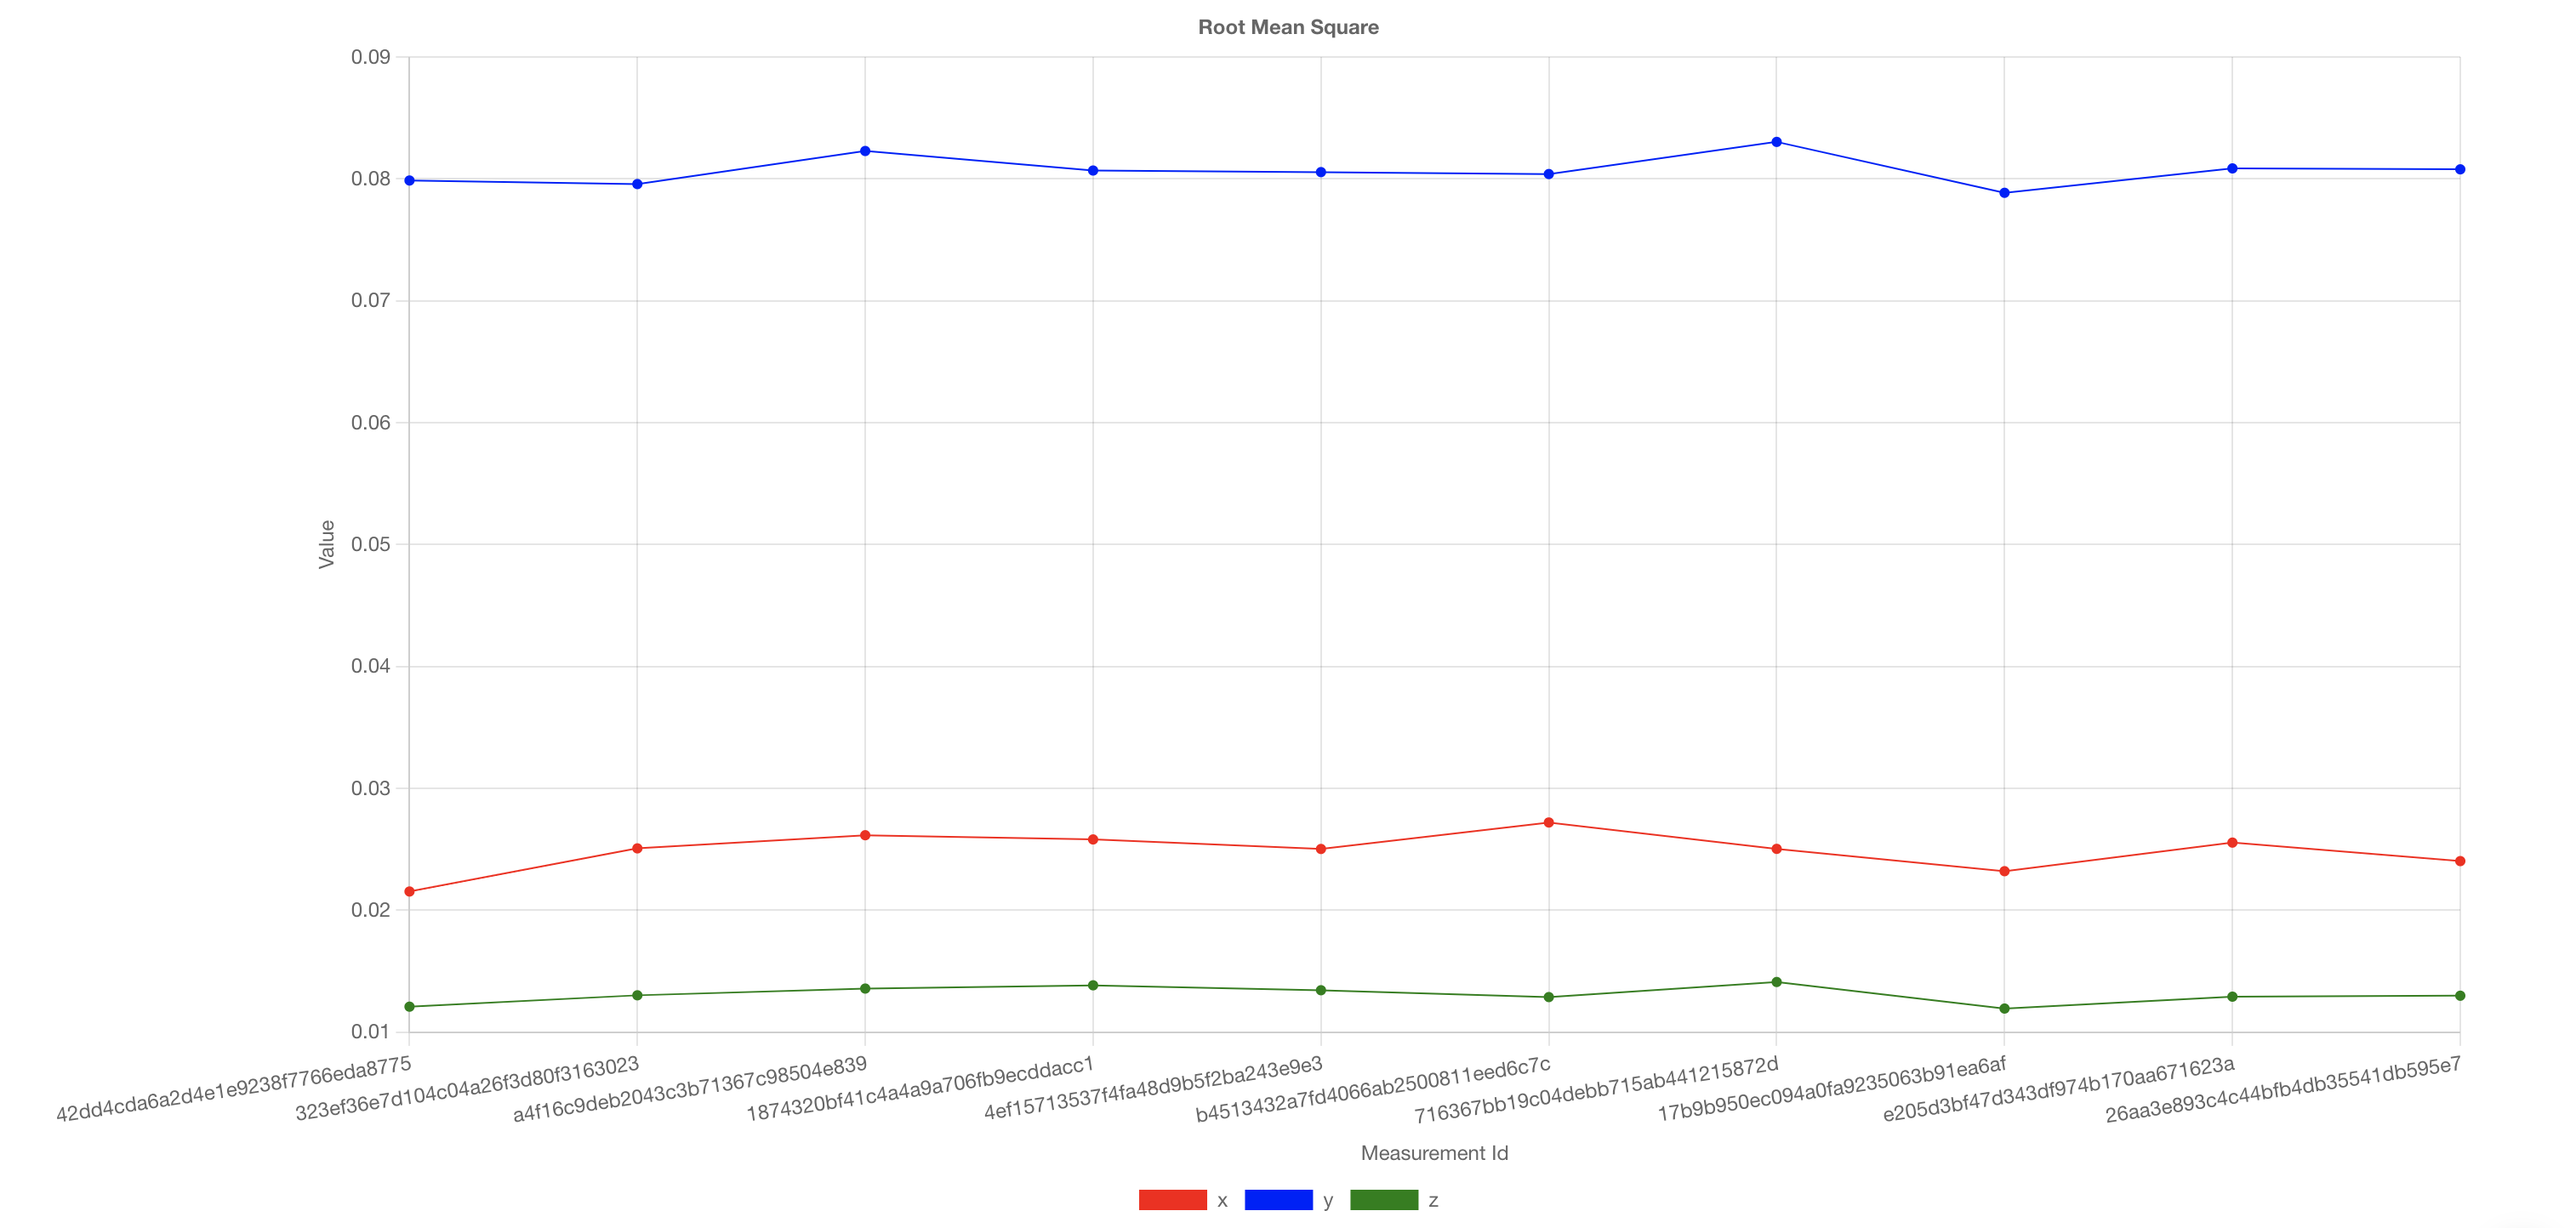
\includegraphics[width=\textwidth]{rms.png}}
\caption{مقادیر ویژگی مربع میانگین ریشه برای همه‌ی اندازه‌گیری‌های یک گره}
\label{fig:rms}
\end{figure}

همانطور که گفته‌شد این ویژگی اطلاعات زیادی را در اختیار ما قرار نمی‌دهد. نکته‌ی قابل توجه دیگر در مورد این ویژگی این است که مقادیر بدست آمده در این ویژگی منسوب به دامنه‌ی زمانی می‌باشد و با توجه به مسئله‌ی کنونی، این ویژگی کاربردی در تحلیل اطلاعات لرزش برای ما نخواهد داشت.


\subsubsection{ویژگی \lr{Power Spectral Density (PSD)}}
ویژگی چگالی طیفی توان یا \lr{PSD} به ما در یافتن مشخصه‌های مبهم موجود در ویژگی‌های مربوط به دامنه‌ی زمانی کمک می‌کند. با ضرب ماتریسی سیگنال لرزش اندازه‌گرفته شده در بعد زمان در یک ماتریس تبدیل کسینوسی گسسته\LTRfootnote{Discrete Cosine Transform (DCT)} به ابعاد $K \times K$، می‌توان بردار ویژگی سیگنال مربوطه را در حوزه‌ی فرکانس بدست آورد. در \cref{eq:psd_feature} طرز محاسبه‌ی این ویژگی را مشاهده می‌کنیم. نکته‌ی قابل توجه در این قسمت این است که بنابر قضیه‌ی پارسوال\LTRfootnote{Parseval's Theorem}، برابری $(r^l_{nm})^2 = \sum_{k = 1}^{K}s^l_{nmk}$ برقرار می‌باشد.

\begin{equation}
\label{eq:psd_feature}
\begin{split} 
s^l_{nm} & = \dfrac{1}{2K}(a^l_{nm} \times W_K)^2\\
s_{nm} &  = \sum_{l \in \{x, y, z\}} s^l_{nm}
\end{split} 
\end{equation}

 پس از این مرحله باید توجه کرد که ویژگی چگالی طیفی توان، یک ویژگی با ابعاد بالا (به اندازه‌ی تعداد نمونه‌ها در یک اندازه‌گیری که در مسئله‌ی ما این عدد برابر با ۶۰ می‌باشد) است که معمولا در هنگام محاسبات ($s^Ts$) منجر به ایجاد ماتریس منفرد\LTRfootnote{Singular Matrix} خواهد شد و در نتیجه برای مسائل رگرسیون دچار مشکل خواهیم شد. از طرف دیگر، این ویژگی به دلیل نوسانات تصادفی زیاد در دامنه آنها در فرکانس به دلیل انحراف اندازه گیری ذاتی در سنسور \lr{MEMS} غیرقابل اتکا است.
 
\subsubsection{ویژگی \lr{Harmonic Peaks Feature}}

برای رفع این مشکلات، ویژگی قله‌های موزون را معرفی می‌کنیم. برای هر اندازه‌گیری با ۶۰ نمونه، این ویژگی عبارت است از ۲۰ تا از بیشترین مقادیر ویژگی \lr{PSD} به همراه فرکانس‌های متناظر با آنها. به عبارت دیگر، این ویژگی به صورت $p_m = \{(f_{mk}, p_{mk})\}_{k=1, ..., n_p}$ تعریف می‌شود که $n_p$ در این مسئله برابر با ۲۰ است.

برای استخراج ویژگی قله‌های موزون، باید دو مرحله را طی کنیم.
\begin{itemize}
\item از بین بردن اثر انحرافات در اندازه‌گیری‌های ویژگی‌ \lr{PSD} با استفاده از عملیات پیچیدگی\LTRfootnote{Convolution} با پنجره‌ی هان\LTRfootnote{Hann Window} که در \cref{eq:hann_window} آورده شده است(در این برابری، $n_h$ اندازه‌ی پنچره است که در مسئله‌ی ما ۱۶ انتخاب شده است). پس از انجام این عملیات، سیگنال ویژگی‌ها هموار\LTRfootnote{Smooth} می‌شود و از این پس می‌توان عملیات جست‌وجو برای بیشترین مقادیر را شروع کرد.

\begin{equation}
\label{eq:hann_window}
w_h(n) = 0.5 (1 - \cos{\dfrac{2\pi n}{n_h - 1}})
\end{equation}

\item پیدا کردن ۲۰ تا از بیشترین مقادیر ویژگی‌های هموارشده از طریق شناسایی نقاطی که مشتق اول سیگنال در آنها از مثبت به منفی، تغییر علامت می‌دهد

\end{itemize}

در \cref{fig:psd} مقادیر ویژگی چگالی طیفی توان و ۲۰ تا از بیشترین قله‌های موزون را برای یکی از اندازه‌گیری‌های منسوب به یک گره، نمایش داده‌ایم.

\begin{figure}[!h]
\centerline{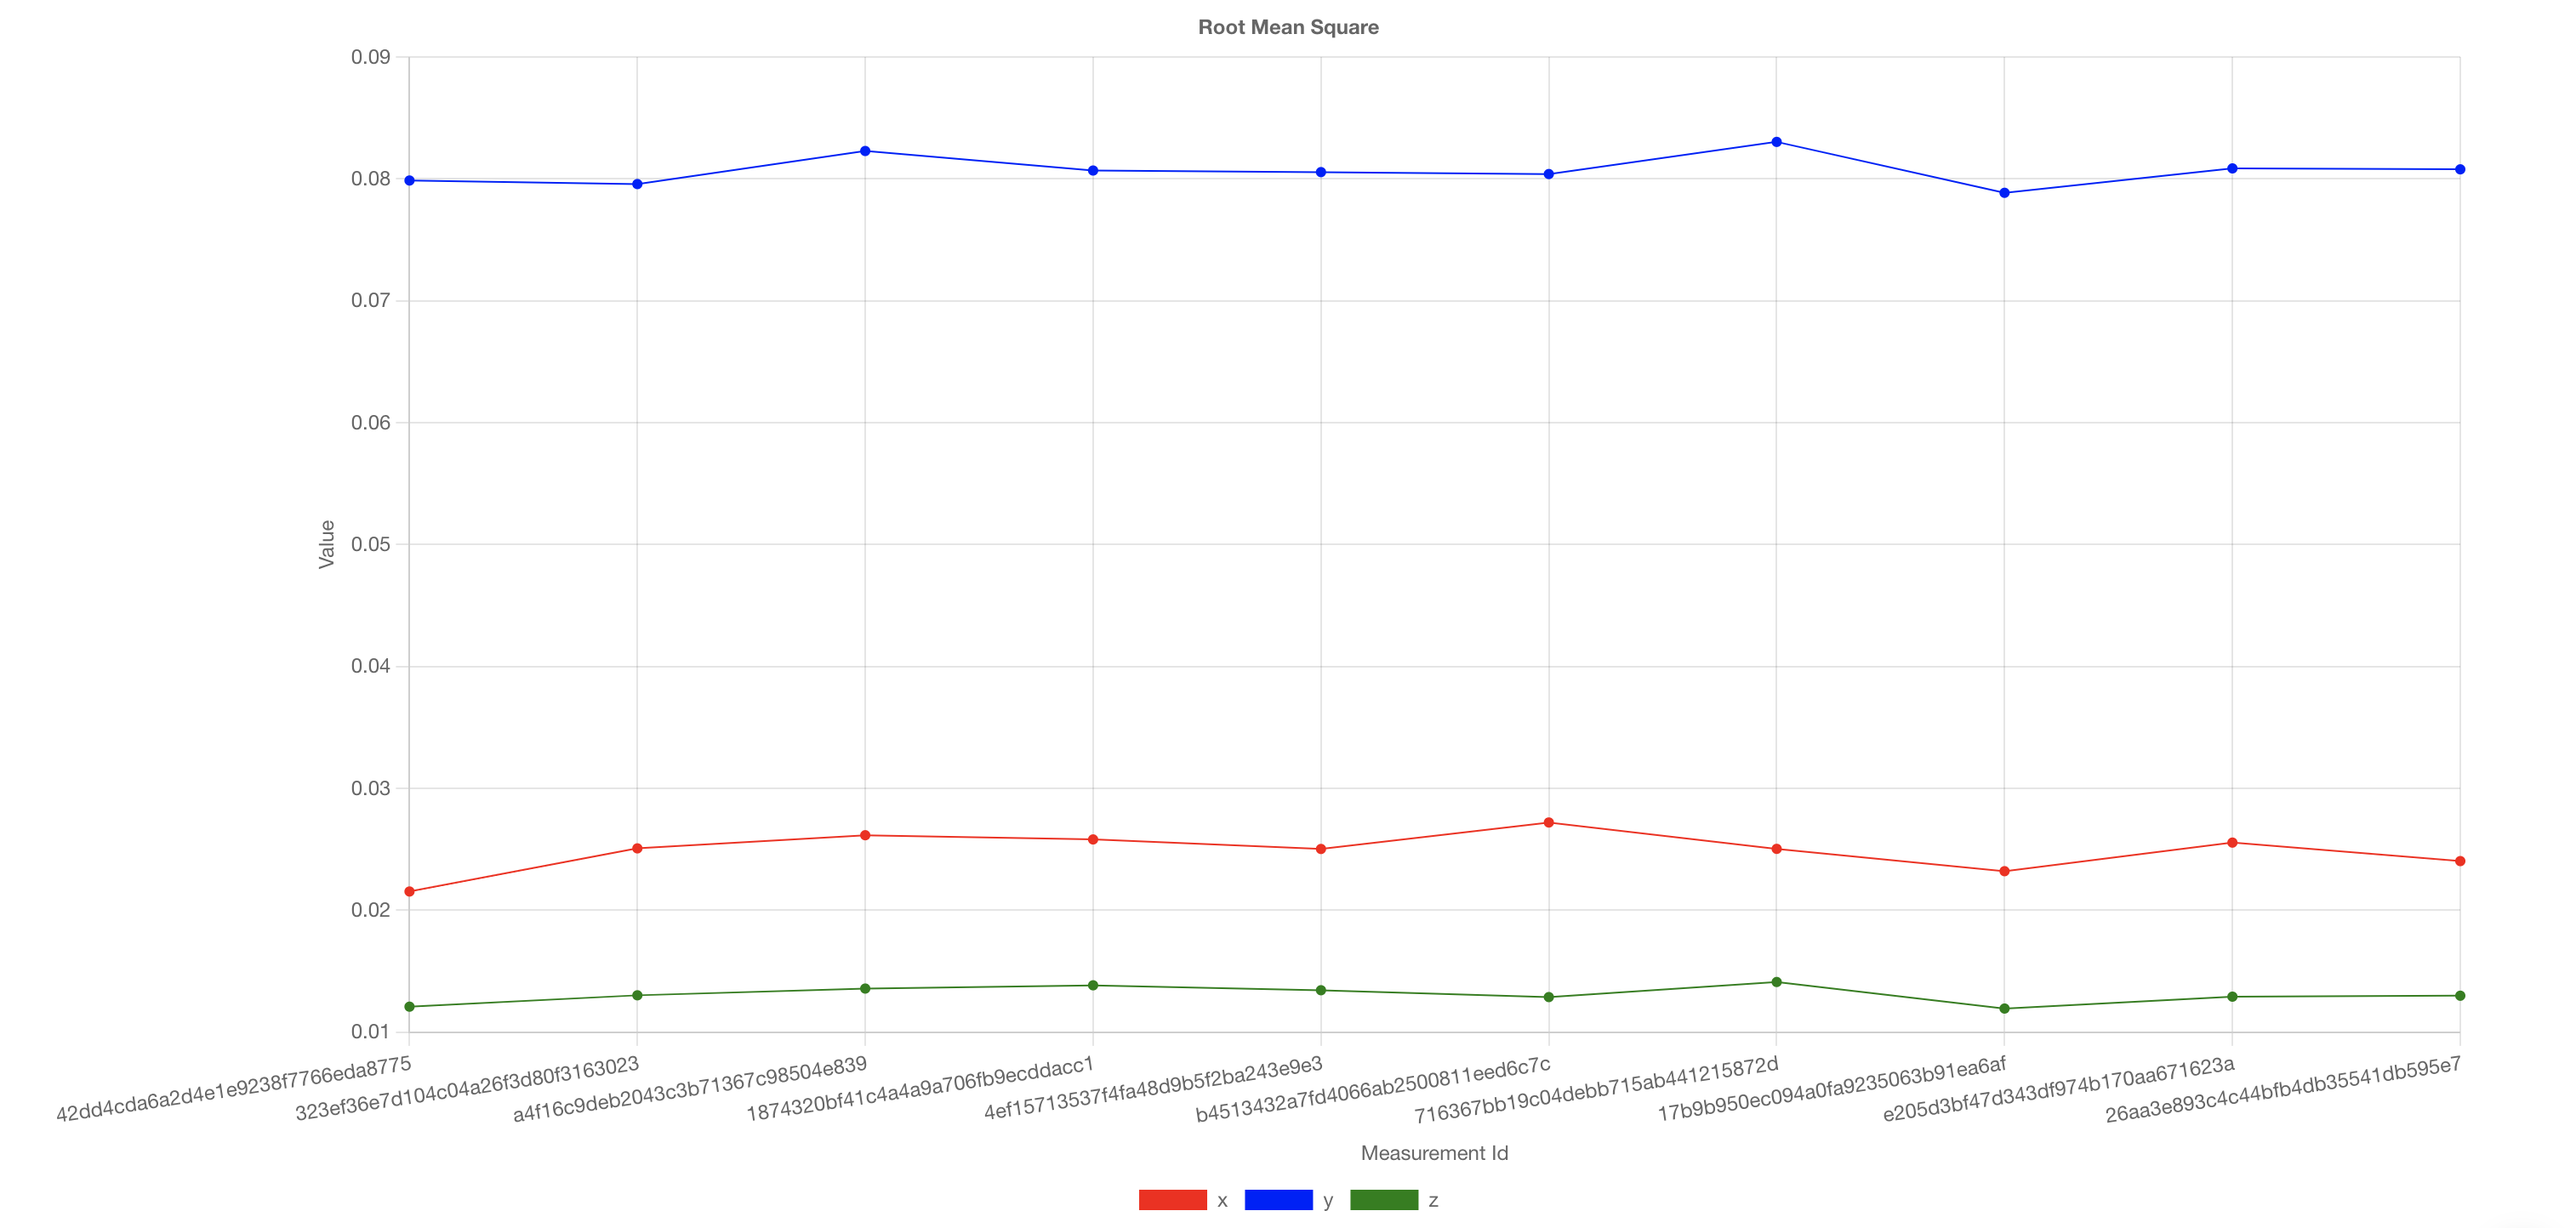
\includegraphics[width=\textwidth]{rms.png}}
\caption{مقادیر ویژگی چگالی طیفی توان و قله‌های موزون برای یک اندازه‌گیری از یک گره}
\label{fig:psd}
\end{figure}

\section{نحوه‌ی یادگیری مدل}
پس از استخراج ویژگی‌ها مناسب، نیازمند آنیم که با تحلیل این ویژگی‌ها به آموزش مدل بپردازیم. برای رسیدن به این مهم باید ابتدا روش مناسبی را برای مقایسه‌ی کمّی بین ویژگی‌های مختلف پیدا کرد. 

\subsection{محاسبه‌ی مشابهت بین وضعیت دستگاه‌ها}
در این مرحله، برای مشخص کردن میزان تفاوت بین دو ویژگی قله‌های موزون $p_i$ و $p_j$، \cref{alg:harmonic_peak_distance} را ارائه می‌دهیم. لازم به ذکر است که خروجی الگوریتم، $D_{ij}$، میزان عددی تفاوت بین ویژگی‌ها است و هرچه این عدد از صفر دورتر باشد، ویژگی‌ها متفاوت‌تر هستند\cite{jung2017vibration}.

\begin{algorithm}
\caption{تشخیص کمّی میزان تفاوت دو ویژگی}
\label{alg:harmonic_peak_distance}
\begin{latin}
\begin{algorithmic}
\Require $p_{max} \gets max(p_n, p_m), f_{max} \gets max(f_n, f_m)$  $\forall (p_n, f_n) \in p_i, \forall (p_m, f_m) \in p_j$
\Ensure $n_h = 16, n_p = 20$
\State $sum \gets 0, cnt \gets 0$
\State $p_n \gets p_n / p_{max},$  $f_n \gets f_n / f_{max},$  $\forall (p_n, f_n) \in p_i$
\State $p_m \gets p_m / p_{max},$  $f_m \gets f_m / f_{max},$  $\forall (p_m, f_m) \in p_j$
\State $queue_i \gets copy(p_i)$
\State $queue_j \gets copy(p_j)$
\While{$queue_i$ is not empty}
\State $(f_i, p_i) \gets queue_i.pop()$
\State {$f* \gets$ do binary search for $f_i$ in $[f_{j1} ... f_{j20}]$}
\If{$|f_i - f_{j*}| \times f_{max} < n_h$}
     \State $(f_{j*}, p_{j*}) \gets queue_j.pop(f_{j*})$
     \State $dist \gets dist + \|(f_i, p_i) - (f_{j*}, p_{j*})\|$
\Else
    \State $dist \gets \|(f_i, p_i)\|$
\EndIf
	\State $sum \gets sum + dist$
	\State $cnt \gets cnt + 1$
\EndWhile
\State $D_{ij} \gets (sum + \sum_{k=1}^{20} p_{jk}) / (cnt + len(p_j))$
\end{algorithmic}
\end{latin}
\end{algorithm}

\subsection{پیاده‌کردن مدل}
پس از طراحی \cref{alg:harmonic_peak_distance} تحلیل ویژگی‌های بدست آمده برای هر اندازه‌گیری را شروع می‌کنیم. نکته‌ی قابل توجه در این الگوریتم این است که این رویه، میزان جریمه‌ی بیشتری را برای مقادیر بیشینه در فرکانس‌های بالاتر در نظر می‌گیرد و این دقیقا همان چیزی است که به ما در شناسایی دستگاه‌های با کارکرد غیر عادی کمک می‌کند. از آنجا که این نوع دستگاه‌ها در فرکانس‌های بالاتر دچار انحرافات شدیدی هستند. در مقابل، دستگاه‌های با کارکرد عادی دارای مقادیر بیشینه‌ی بیشتر در فرکانس‌های پایین‌تر هستند.

با یک فرض پایه، توضیح نحوه‌ی یادگیری مدل را شروع می‌کنیم و آن این است که کلیه‌ی دستگاه‌ها به مرور زمان و با کار بیشتر، از حالت نویی دور می‌شوند. به عبارت دیگر، با گذشت زمان، هر دستگاه از وضعیت دستگاه تازه و آماده به کار دورتر می‌شود. برای این منظور، پارامتر $D_a$ را برای تحلیل دستگاه‌ها معرفی می‌کنیم که عبارت‌است از میزان متفاوت بودن دستگاه مورد نظر با یک 
دستگاه نو (کلاس کاری $A$ در \cref{table:node_state_labels}). تا زمانیکه هیچ نگهداری‌ای برای دستگاه صورت نگیرد، $D_a$ به مرور زمان به صورت یکنواخت افزایش می‌یابد.

\subsubsection{الگوریتم \lr{RANSAC}}

برای یادگیری این مدل خطی و پیش‌بینی زمان سرویس دستگاه‌ها از رویکرد اجماع نمونه‌ی تصادفی\LTRfootnote{RANdom SAmple Consensus (RANSAC)} یا به اختصار \lr{RANSAC} استفاده می‌کنیم. این الگوریتم، به صورت بازگشتی، مدل خطی‌ای بر اساس داده‌های آموزشی درست می‌کند و نکته‌ی قابل توجه این الگوریتم این است که توانایی تشخیص و در نظر نگرفتن داده‌های پرت را دارد و از این رو بسیار مناسب استفاده در این مسئله است. به طور کلی روند ایجاد مدل در این الگوریتم به صورت زیر است\cite{derpanis2010overview}:

\begin{enumerate}

\item به صورت تصادفی حداقل تعداد نقاط لازم، برای پیداکردن پارامترهای مدل مشخص می‌شود.
\item پارامتر‌های مدل بدست آورده می‌شوند.
\item از میان کل نقاط، تعداد نقاطی که با میزان تحمل از قبل تعیین شده‌ی $\epsilon$ شامل مدل هستند، حساب می‌شوند.
\item اگر نسبت نقاط مشمول در مدل به تعداد کل نقاط از یک مقدار از پیش‌ تعیین‌شده‌ی $\tau$ بیشتر شد، پارامتر‌های مدل دوباره با کمک نقاط مشمول حدس زده می‌شوند و الگوریتم پایان می‌یابد.
\item در غیر این صورت، مرحله‌ی ۱ تا ۴ تا حداکثر $N$ بار تکرار می‌شود.

\end{enumerate}

جهت پیش‌بینی میزان عمر مفید باقی‌مانده، الگوریتم ما ابتدا آستانه‌ی $D_a$ را برای دو کلاس کاری $B, C$ و $D$ حساب می‌کند. این آستانه از طریق کمینه کردن میزان خطا در طبقه‌بندی دستگاه‌های این دو کلاس مشخص می‌شود. پس از تعیین این آستانه، الگوریتم با بررسی مدل خطی بدست‌آمده از \lr{RANSAC}، میزان عمر مفید دستگاه مربوطه را خروجی‌ می‌دهد.

در \cref{fig:ransac_model}\cite{jung2017vibration} دو مدل برای پیش‌بینی میزان عمر مفید باقی‌مانده، آموزش داده‌شده است. محور افقی زمان اندازه‌گیری‌ها بر حسب روز و محور عمودی فاصله‌ی ویژگی‌های دستگاه‌ها با ویژگی دستگاه‌های سالم و نو است. همچنین خط بنفش‌رنگ، آستانه‌ی ورود دستگاه از کلاس دستگاه‌های سالم به کلاس دستگاه‌های معیوب می‌باشد (این مقدار آستانه در شکل برابر با ۰/۲۱ است). برای پیش‌بینی عمر باقی‌مانده‌ی هر دستگاه ابتدا میزان تعلق مقادیر $D_a$ برای آن دستگاه در دو مدل محاسبه می‌شود. سپس این حد آستانه با مدلی که دستگاه بیشترین تعلق را به آن دارد تلاقی داده می‌شود. در نهایت فاصله‌ی زمان اندازه‌گیری با نقطه‌ی تلاقی، برابر با عمر مفید باقی‌مانده‌ی دستگاه مورد نظر بر حسب روز است.

\begin{figure}[!h]
\centerline{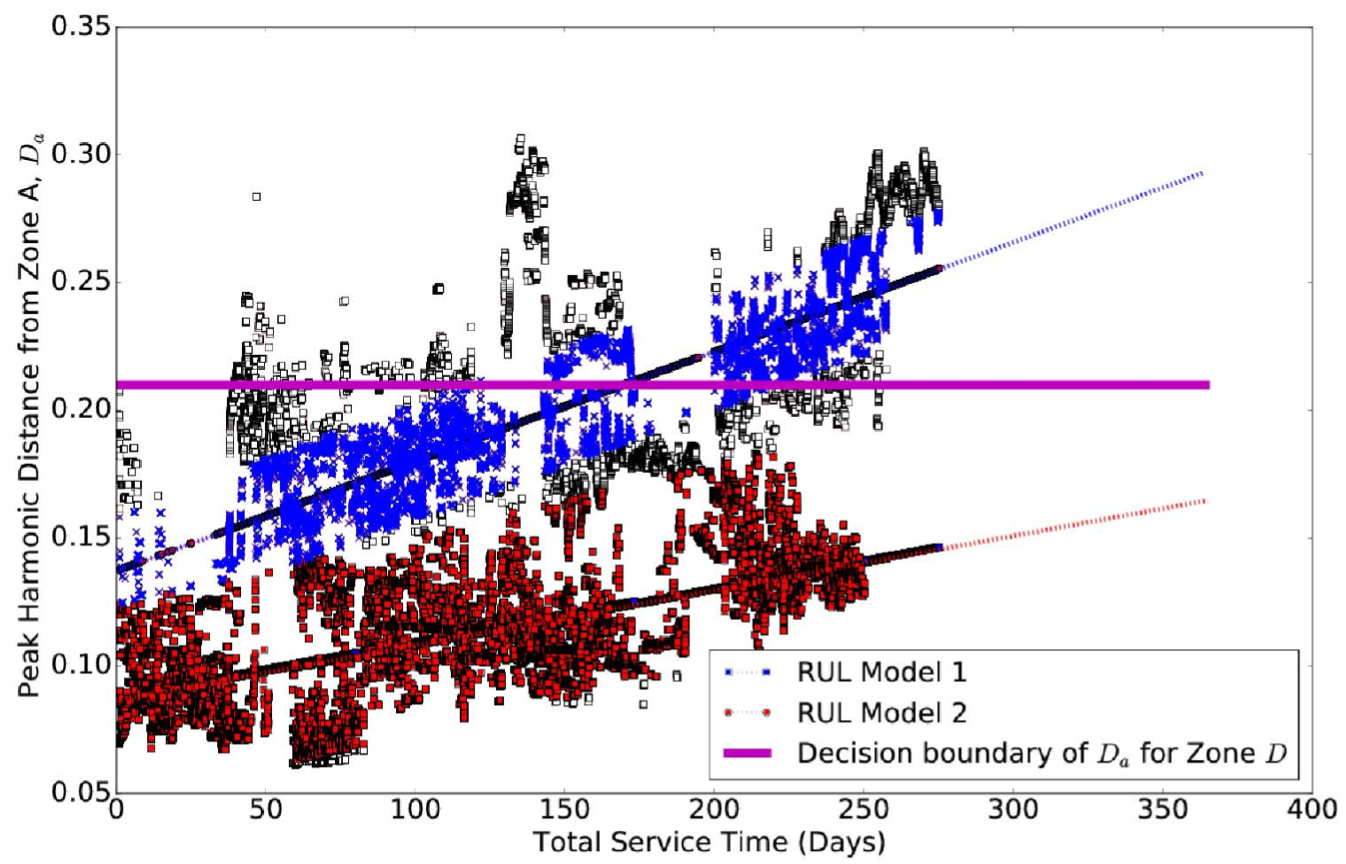
\includegraphics[width=0.8\textwidth]{ransac_model.png}}
\caption{دو مدل یادگیری ماشین برای مسئله‌ی پیش‌بینی میزان عمر مفید باقی‌مانده\cite{jung2017vibration}}
\label{fig:ransac_model}
\end{figure}

\section{جمع‌بندی و نتیجه‌گیری}
این بخش به طور دقیق روند یادگیری ماشین از اطلاعات لرزش گره‌ها را نشان داد. مشخص شد که داده‌های جمع‌آوری شده ابتدا به کمک پیش‌پردازنده که شامل هنجارکننده، تشخیص‌دهنده‌ی داده‌ی پرت و استخراج‌کننده‌ی ویژگی‌های آماده پردازش است، پالایش شده و سپس تحویل واحد یادگیری ماشین می‌شود. در این مرحله این واحد ابتدا با هموار کردن و سپس با انتخاب کردن ۲۰ تا از بیشترین مقادیر موزون ویژگی \lr{PSD} برای هر اندازه‌گیری، اقدام به محاسبه‌ی میزان شباهت این اندازه‌گیری‌ها به اندازه‌گیری‌های یک دستگاه سالم می‌کند و بنا به میزان شباهت یا تفاوت با آن، پیش‌بینی مربوط به طول عمر باقی‌مانده‌ی گره را خروجی خواهد داد.